


\tikzset{every picture/.style={line width=0.75pt}} %set default line width to 0.75pt        

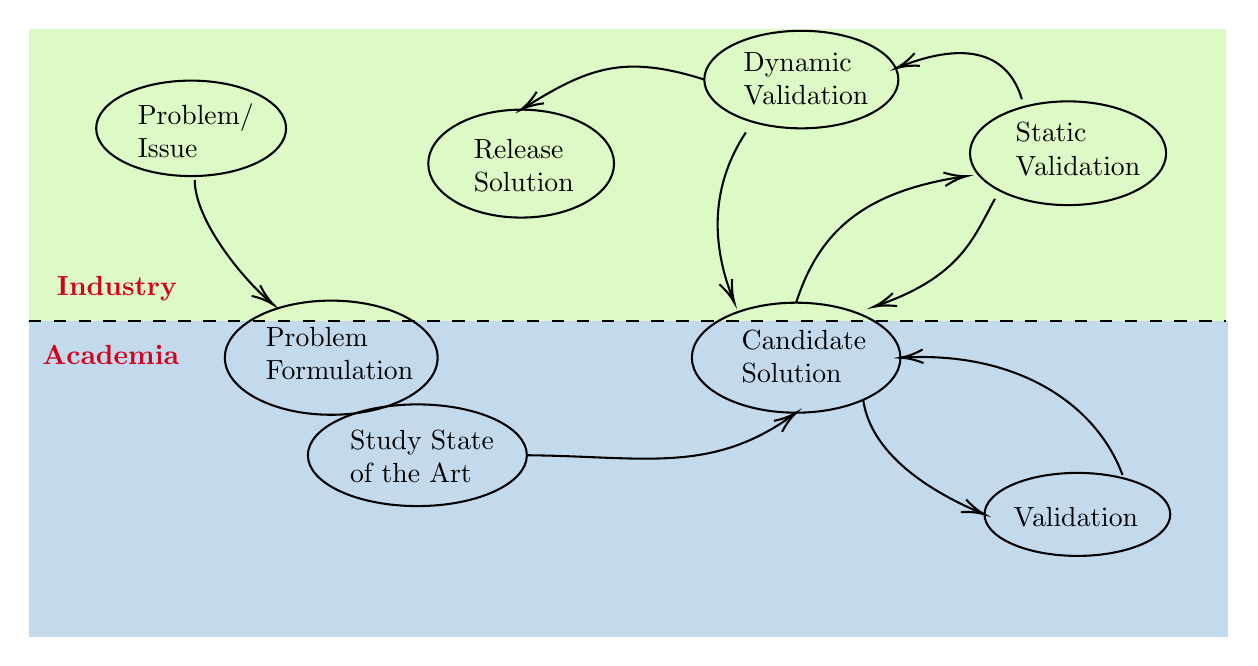
\begin{tikzpicture}[x=0.75pt,y=0.75pt,yscale=-1,xscale=1]
%uncomment if require: \path (0,300); %set diagram left start at 0, and has height of 300

%Shape: Rectangle [id:dp578818274976289] 
\draw  [draw opacity=0][fill={rgb, 255:red, 221; green, 250; blue, 198 }  ,fill opacity=1 ] (12.5,1) -- (589.44,1) -- (589.44,142) -- (12.5,142) -- cycle ;
%Shape: Rectangle [id:dp8699585076120131] 
\draw  [draw opacity=0][fill={rgb, 255:red, 195; green, 218; blue, 236 }  ,fill opacity=1 ][dash pattern={on 0.84pt off 2.51pt}] (12.5,142) -- (590.5,142) -- (590.5,294) -- (12.5,294) -- cycle ;
%Straight Lines [id:da676387418417167] 
\draw  [dash pattern={on 4.5pt off 4.5pt}]  (12.5,142) -- (589.44,142) ;


%Shape: Ellipse [id:dp6781348387425088] 
\draw   (107,159.5) .. controls (107,144.31) and (129.95,132) .. (158.25,132) .. controls (186.55,132) and (209.5,144.31) .. (209.5,159.5) .. controls (209.5,174.69) and (186.55,187) .. (158.25,187) .. controls (129.95,187) and (107,174.69) .. (107,159.5) -- cycle ;
%Shape: Ellipse [id:dp2708464373524213] 
\draw   (147,206.5) .. controls (147,192.97) and (170.62,182) .. (199.75,182) .. controls (228.88,182) and (252.5,192.97) .. (252.5,206.5) .. controls (252.5,220.03) and (228.88,231) .. (199.75,231) .. controls (170.62,231) and (147,220.03) .. (147,206.5) -- cycle ;
%Shape: Ellipse [id:dp21542593477891825] 
\draw   (332,159.5) .. controls (332,144.86) and (354.5,133) .. (382.25,133) .. controls (410,133) and (432.5,144.86) .. (432.5,159.5) .. controls (432.5,174.14) and (410,186) .. (382.25,186) .. controls (354.5,186) and (332,174.14) .. (332,159.5) -- cycle ;
%Shape: Ellipse [id:dp4564599934587261] 
\draw   (473,235) .. controls (473,223.95) and (493.04,215) .. (517.75,215) .. controls (542.46,215) and (562.5,223.95) .. (562.5,235) .. controls (562.5,246.05) and (542.46,255) .. (517.75,255) .. controls (493.04,255) and (473,246.05) .. (473,235) -- cycle ;
%Shape: Ellipse [id:dp3265553941370425] 
\draw   (45,49) .. controls (45,36.3) and (65.48,26) .. (90.75,26) .. controls (116.02,26) and (136.5,36.3) .. (136.5,49) .. controls (136.5,61.7) and (116.02,72) .. (90.75,72) .. controls (65.48,72) and (45,61.7) .. (45,49) -- cycle ;
%Shape: Ellipse [id:dp47231378471298047] 
\draw   (205,66) .. controls (205,51.64) and (225.04,40) .. (249.75,40) .. controls (274.46,40) and (294.5,51.64) .. (294.5,66) .. controls (294.5,80.36) and (274.46,92) .. (249.75,92) .. controls (225.04,92) and (205,80.36) .. (205,66) -- cycle ;
%Shape: Ellipse [id:dp9535240877112273] 
\draw   (466,61) .. controls (466,47.19) and (487.15,36) .. (513.25,36) .. controls (539.35,36) and (560.5,47.19) .. (560.5,61) .. controls (560.5,74.81) and (539.35,86) .. (513.25,86) .. controls (487.15,86) and (466,74.81) .. (466,61) -- cycle ;
%Shape: Ellipse [id:dp012300500225925659] 
\draw   (338,25.5) .. controls (338,12.52) and (358.93,2) .. (384.75,2) .. controls (410.57,2) and (431.5,12.52) .. (431.5,25.5) .. controls (431.5,38.48) and (410.57,49) .. (384.75,49) .. controls (358.93,49) and (338,38.48) .. (338,25.5) -- cycle ;
%Curve Lines [id:da18609872916572134] 
\draw    (92.5,74) .. controls (92.5,92.43) and (114.14,120.27) .. (129.13,132.87) ;
\draw [shift={(130.5,134)}, rotate = 218.66] [color={rgb, 255:red, 0; green, 0; blue, 0 }  ][line width=0.75]    (10.93,-3.29) .. controls (6.95,-1.4) and (3.31,-0.3) .. (0,0) .. controls (3.31,0.3) and (6.95,1.4) .. (10.93,3.29)   ;

%Curve Lines [id:da8707215769538176] 
\draw    (252.5,206.5) .. controls (308.93,207) and (341.59,215.82) .. (381.05,186.89) ;
\draw [shift={(382.25,186)}, rotate = 503.13] [color={rgb, 255:red, 0; green, 0; blue, 0 }  ][line width=0.75]    (10.93,-3.29) .. controls (6.95,-1.4) and (3.31,-0.3) .. (0,0) .. controls (3.31,0.3) and (6.95,1.4) .. (10.93,3.29)   ;

%Curve Lines [id:da6178019241672817] 
\draw    (414.5,179.5) .. controls (418.38,208.12) and (451.43,225.91) .. (471.2,234.25) ;
\draw [shift={(473,235)}, rotate = 202.31] [color={rgb, 255:red, 0; green, 0; blue, 0 }  ][line width=0.75]    (10.93,-3.29) .. controls (6.95,-1.4) and (3.31,-0.3) .. (0,0) .. controls (3.31,0.3) and (6.95,1.4) .. (10.93,3.29)   ;

%Curve Lines [id:da6452800872792407] 
\draw    (539.5,216) .. controls (526.63,181.35) and (488.28,156.5) .. (434.15,159.4) ;
\draw [shift={(432.5,159.5)}, rotate = 356.36] [color={rgb, 255:red, 0; green, 0; blue, 0 }  ][line width=0.75]    (10.93,-3.29) .. controls (6.95,-1.4) and (3.31,-0.3) .. (0,0) .. controls (3.31,0.3) and (6.95,1.4) .. (10.93,3.29)   ;

%Curve Lines [id:da006231701109337573] 
\draw    (382.25,133) .. controls (393.39,98.35) and (415.06,79.38) .. (463.04,72.21) ;
\draw [shift={(464.5,72)}, rotate = 531.87] [color={rgb, 255:red, 0; green, 0; blue, 0 }  ][line width=0.75]    (10.93,-3.29) .. controls (6.95,-1.4) and (3.31,-0.3) .. (0,0) .. controls (3.31,0.3) and (6.95,1.4) .. (10.93,3.29)   ;

%Curve Lines [id:da3086608797307422] 
\draw    (478,83) .. controls (467.66,101.72) and (461.68,120.43) .. (421.37,134.37) ;
\draw [shift={(419.5,135)}, rotate = 341.57] [color={rgb, 255:red, 0; green, 0; blue, 0 }  ][line width=0.75]    (10.93,-3.29) .. controls (6.95,-1.4) and (3.31,-0.3) .. (0,0) .. controls (3.31,0.3) and (6.95,1.4) .. (10.93,3.29)   ;

%Curve Lines [id:da48274664662536704] 
\draw    (491,35) .. controls (484.6,13.33) and (465.1,6.21) .. (432.02,19.38) ;
\draw [shift={(430.5,20)}, rotate = 337.62] [color={rgb, 255:red, 0; green, 0; blue, 0 }  ][line width=0.75]    (10.93,-3.29) .. controls (6.95,-1.4) and (3.31,-0.3) .. (0,0) .. controls (3.31,0.3) and (6.95,1.4) .. (10.93,3.29)   ;

%Curve Lines [id:da9832521962719682] 
\draw    (358,51) .. controls (341.83,75.5) and (340.55,102.88) .. (351.8,131.26) ;
\draw [shift={(352.5,133)}, rotate = 247.51999999999998] [color={rgb, 255:red, 0; green, 0; blue, 0 }  ][line width=0.75]    (10.93,-3.29) .. controls (6.95,-1.4) and (3.31,-0.3) .. (0,0) .. controls (3.31,0.3) and (6.95,1.4) .. (10.93,3.29)   ;

%Curve Lines [id:da11627273776087521] 
\draw    (338,25.5) .. controls (299.09,13.19) and (282.02,19.79) .. (251.17,39.11) ;
\draw [shift={(249.75,40)}, rotate = 327.78999999999996] [color={rgb, 255:red, 0; green, 0; blue, 0 }  ][line width=0.75]    (10.93,-3.29) .. controls (6.95,-1.4) and (3.31,-0.3) .. (0,0) .. controls (3.31,0.3) and (6.95,1.4) .. (10.93,3.29)   ;


% Text Node
\draw (52,158) node  [align=left] {\textcolor[rgb]{0.82,0.01,0.11}{\textbf{Academia}}};
% Text Node
\draw (55,126) node  [align=left] {\textbf{\textcolor[rgb]{0.82,0.01,0.11}{Industry}}};
% Text Node
\draw (93,50) node  [align=left] {Problem/\\Issue};
% Text Node
\draw (202,207) node  [align=left] {Study State\\of the Art};
% Text Node
\draw (162.25,157.5) node  [align=left] {Problem \\Formulation};
% Text Node
\draw (251,67) node  [align=left] {Release\\Solution};
% Text Node
\draw (387,25) node  [align=left] {Dynamic\\Validation};
% Text Node
\draw (518,59) node  [align=left] {Static\\Validation};
% Text Node
\draw (386,159) node  [align=left] {Candidate\\Solution};
% Text Node
\draw (517,244) node  [align=left] {Validation\\};


\end{tikzpicture}